
\chapter{Generalizations}











\section{Parking with overlap}

We now look at the problem of parking with overlap, which is of practical 
interest in the context of particle adsorption (see \cite{roach2000parking}). 
Let $\phi$ denote the region of overlap, with $0 \leq \phi \leq 1$. We 
therefore have an exclusion zone around the centre of a car of length 
$1 - \phi$. Our problem is now the process of finding parking spots where 
exclusion zones do not overlap. This is equivalent to the parking problem 
but instead of dealing with cars of unit length we park the exclusion zones 
of length $1 - \phi$. We introduce a new gap density function 
$P_{\phi}(x, t)$ taking this into account, with allowed overlap $\phi$. \bigskip

Let $\bar{x}$ denote the distance between cars, and $x$ denote the distance 
between exclusion zones. Clearly $\bar{x} = x - \phi$. From this we can see 
that the distance between exclusion zones is always positive, but the distance 
between cars can be negative, in the case of overlap. \bigskip

Similar to the Kinetic approach, we define a rate equation for the creation and 
destruction of gaps for the overlap case: \bigskip

\begin{eqnarray*}
	\frac{\partial P_{\phi}(x, t)}{\partial t} = 
	\begin{dcases}
		2 \int_{x + 1 - \phi}^{\infty} P_{\phi}(y, t) dy                                   & \text{for } x < 1 - \phi \\\\
		-(x - 1 + \phi) P_{\phi}(x, t) + 2 \int_{x + 1 - \phi}^{\infty} P_{\phi}(y, t) dy  & \text{for } x \geq 1 - \phi
	\end{dcases}
\end{eqnarray*}\medskip

We take a similar approach to solving the above as was taken in the Kinetic 
approach. i.e. if we let: \bigskip

\[
	P_{\phi}(x, t) = A(t) e^{-(x - 1 + \phi)t}
\]\medskip 

and make the further substitution $A(t) = t^2 F_{\phi}(t)$, we find that: \bigskip

\[
	F_{\phi}(t) = \exp \left( -2 \int_{0}^{t} \frac{(1 - e^{-(1 - \phi)\tau})}{\tau} d\tau \right)
\]\medskip

The gap density function for gaps between exclusion zones becomes: \bigskip

\begin{eqnarray*}
	P_{\phi}(x, t) = 
	\begin{dcases}
		2 \int_{0}^{t} \tau F_{\phi}(\tau) e^{-x\tau} d\tau		& \text{for } x < 1 - \phi \\\\
		t^2 F_{\phi}(t) e^{-(x - 1 + \phi)t}					& \text{for } x \geq 1 - \phi 
	\end{dcases}
\end{eqnarray*}\medskip

and coverage by exclusion zone becomes: \bigskip

\begin{eqnarray*}
			\frac{d \theta_{\phi}}{dt} & = & (1 - \phi) F_{\phi}(t) \\\\
	 \therefore \quad \theta_{\phi}(t) & = & (1 - \phi) \int_{0}^{t} F_{\phi}(\tau) d\tau
\end{eqnarray*}\medskip

In figure \ref{fig:cfo1} we see the behaviour of the coverage function for 
different values of $\phi$. As is to be expected, the coverage tends towards 
$C_{R}$ as $t$ increases. \bigskip

\begin{figure}[h!]
	\centering
	%	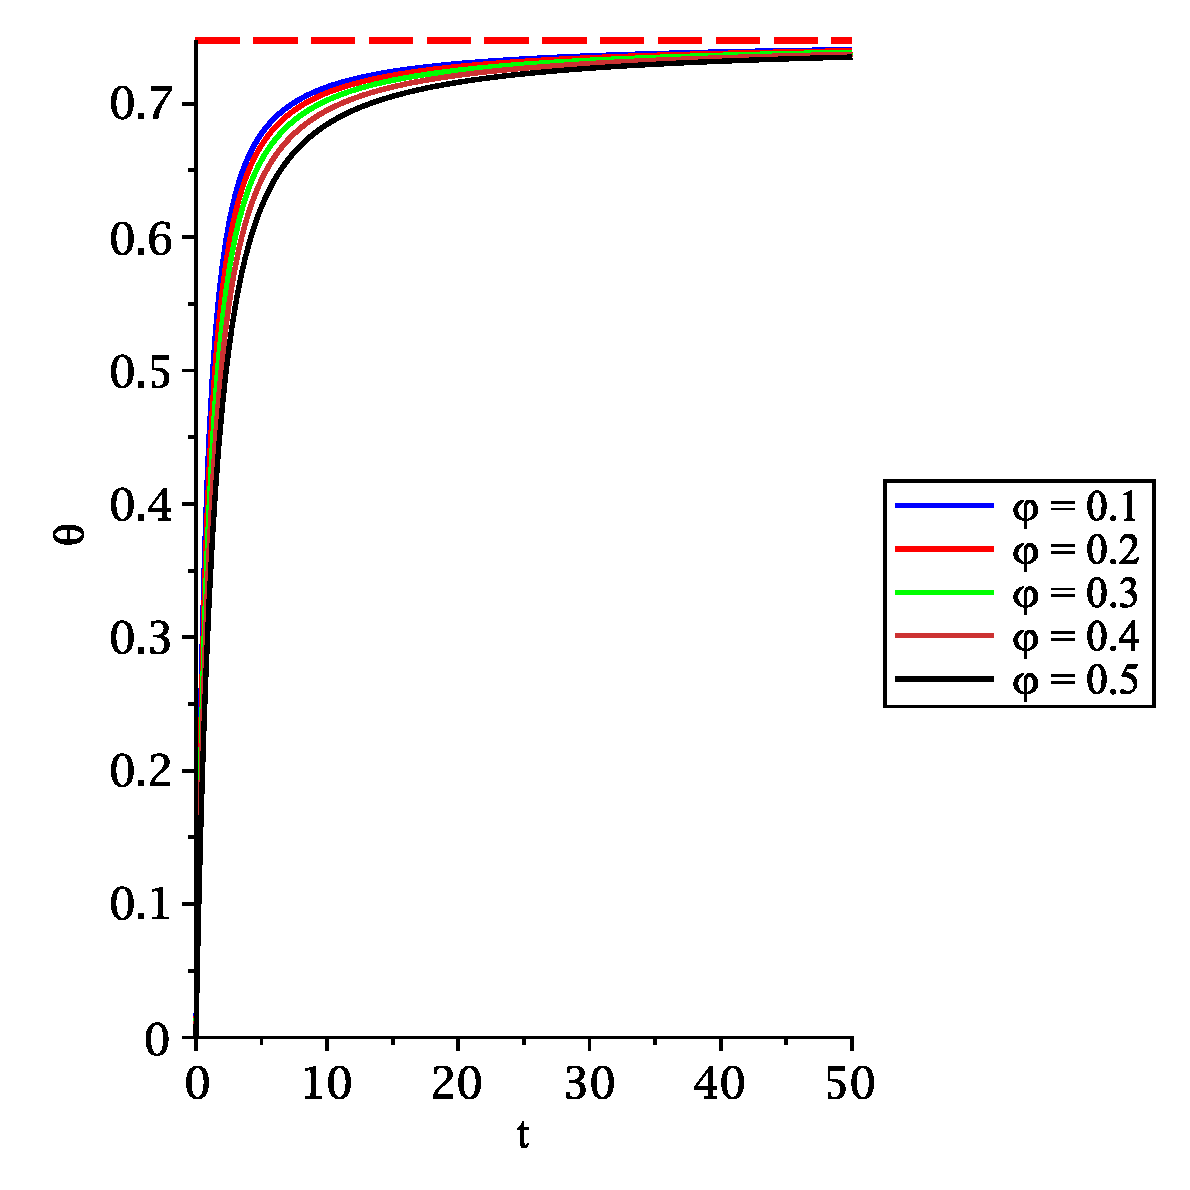
\includegraphics[scale = 0.35]{coverage_overlap_01.eps}
	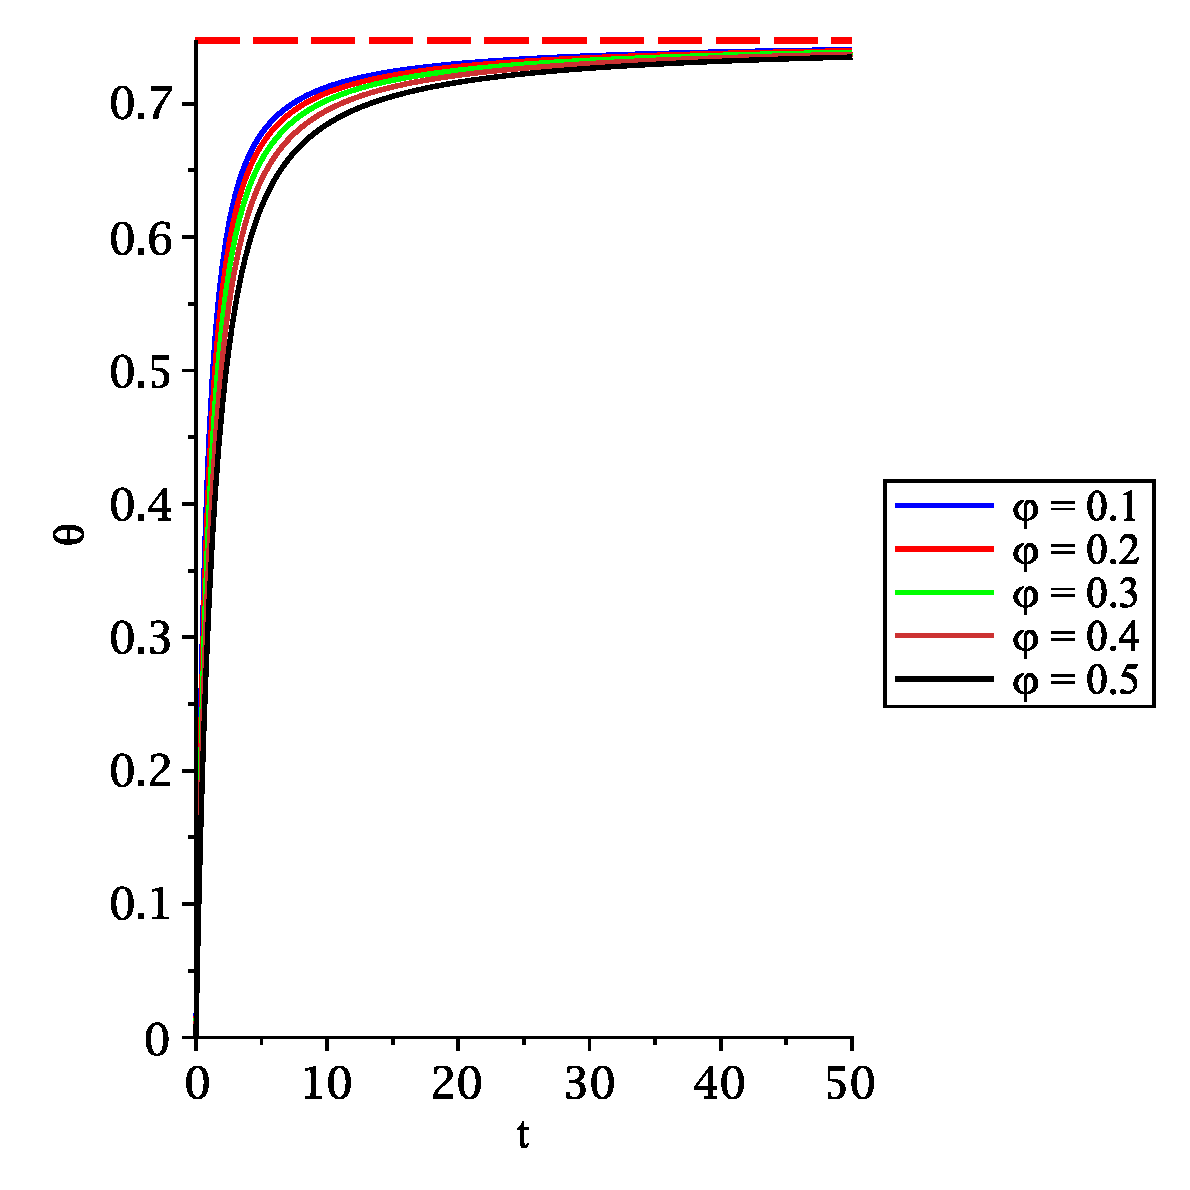
\includegraphics[width=\textwidth]{coverage_overlap_01.eps}
	\caption{The coverage function - overlap case}
	\label{fig:cfo1}
\end{figure}\medskip

The gap density function for gaps between cars, $\bar{x} = x - \phi$,  becomes: \bigskip

\begin{eqnarray*}
	Q_{\phi}(\bar{x}, t) = 
	\begin{dcases}
		2 \int_{0}^{t} \tau F_{\phi}(\tau) e^{-(\bar{x} + \phi)\tau} d\tau			& \text{for } \bar{x} < 1 - 2 \phi \\\\
		t^2 F_{\phi}(t) e^{-(\bar{x} - 1 + 2 \phi)t}								& \text{for } \bar{x} \geq 1 - 2 \phi 
	\end{dcases}
\end{eqnarray*}\medskip

and coverage by cars becomes: \bigskip

\[
	\Theta_{\phi}(t) = 1 - \int_{0}^{\infty} \bar{x} Q_{\phi}(\bar{x}, t) d\bar{x}
\]\medskip

Differentiating with respect to $t$ we get: \bigskip

\begin{eqnarray*}
	\frac{d \Theta_{\phi}}{dt} & = & -\frac{\partial}{\partial t} \int_{0}^{\infty} \bar{x} Q_{\phi}(\bar{x}, t) d\bar{x} \\\\
							   & = & -\frac{\partial}{\partial t} \left( \int_{0}^{1 - 2 \phi} \bar{x} Q_{\phi}(\bar{x}, t) d\bar{x} 
										- \int_{1 - 2 \phi}^{\infty} \bar{x} Q_{\phi}(\bar{x}, t) d\bar{x} \right) \\\\
							   & = & -\frac{\partial}{\partial t} \left( \int_{0}^{1 - 2 \phi} \bar{x} \left( 2 \int_{0}^{t} \tau F_{\phi}(\tau) e^{-(\bar{x} + \phi)\tau} d\tau \right) d\bar{x} 
										- \int_{1 - 2 \phi}^{\infty} \bar{x} t^2 F_{\phi}(t) e^{-(\bar{x} - 1 + 2 \phi)t} d\bar{x} \right) \\\\
							   & = & -\frac{\partial}{\partial t} \int_{0}^{1 - 2 \phi} \bar{x} \left( 2 \int_{0}^{t} \tau F_{\phi}(\tau) e^{-(\bar{x} + \phi)\tau} d\tau \right) d\bar{x} 
										- \frac{\partial}{\partial t} \int_{1 - 2 \phi}^{\infty} \bar{x} t^2 F_{\phi}(t) e^{-(\bar{x} - 1 + 2 \phi)t} d\bar{x} 
\end{eqnarray*}\medskip

for $\phi < \frac{1}{2}$. We will deal with each part of the right hand side separately. Starting with the first part: \bigskip

\begin{eqnarray*}
	-\frac{\partial}{\partial t} \int_{0}^{1 - 2 \phi} \bar{x} \left( 2 \int_{0}^{t} \tau F_{\phi}(\tau) e^{-(\bar{x} + \phi)\tau} d\tau \right) d\bar{x} & = & 
			-\int_{0}^{1 - 2 \phi} \bar{x} \left( 2 \frac{\partial}{\partial t} \int_{0}^{t} \tau F_{\phi}(\tau) e^{-(\bar{x} + \phi)\tau} d\tau \right) d\bar{x} \\\\
																																						  & = & 
			-\int_{0}^{1 - 2 \phi} \bar{x} 2 t F_{\phi}(t) e^{-(\bar{x} + \phi)t} d\bar{x} \\\\
																																						  & = & 
			-2 t F_{\phi}(t) e^{-\phi t} \int_{0}^{1 - 2 \phi} \bar{x} e^{-\bar{x} t} d\bar{x} \\\\
																																						  & = & 
			-2 t F_{\phi}(t) e^{-\phi t} \left[ - \frac{(1 - 2 \phi) e^{-(1 - 2 \phi)t}}{t} - \frac{e^{-(1 - 2 \phi)t}}{t^2} + \frac{1}{t^2} \right] \\\\
																																						  & = & 
			2 F_{\phi}(t) (1 - 2 \phi) e^{-(1 - \phi) t} + \frac{2 F_{\phi}(t) e^{-(1 - \phi)t}}{t} - \frac{2 F_{\phi}(t) e^{-\phi t}}{t}
\end{eqnarray*}\medskip

moving on to the second part: \bigskip

\begin{eqnarray*}
	-\frac{\partial}{\partial t} \int_{1 - 2 \phi}^{\infty} \bar{x} t^2 F_{\phi}(t) e^{-(\bar{x} - 1 + 2 \phi)t} d\bar{x} & = & 
			-\int_{1 - 2 \phi}^{\infty} \bar{x} \frac{\partial}{\partial t} \left( t^2 F_{\phi}(t) e^{-(\bar{x} - 1 + 2 \phi)t} \right) d\bar{x} \\\\
																														  & = & 
			-\int_{1 - 2 \phi}^{\infty} \bar{x} \frac{\partial}{\partial t} \left( t^2 F_{\phi}(t) e^{(1 - 2 \phi)t} e^{-\bar{x} t} \right) d\bar{x} 
\end{eqnarray*}\medskip

The differential within the integral is: \bigskip

\begin{eqnarray*}
	\frac{\partial}{\partial t} \left( t^2 F_{\phi}(t) e^{(1 - 2 \phi)t} e^{-\bar{x} t} \right) & = & 2 t F_{\phi}(t) e^{(1 - 2 \phi)t} e^{-\bar{x} t} \\\\
																								&   & + t^2 F_{\phi}^{\prime}(t) e^{(1 - 2 \phi)t} e^{-\bar{x} t} \\\\
																								&   & + t^2 F_{\phi}(t) (1 - 2 \phi) e^{(1 - 2 \phi)t} e^{-\bar{x} t} \\\\
																								&   & - t^2 F_{\phi}(t) e^{(1 - 2 \phi)t} \bar{x} e^{-\bar{x} t} 
\end{eqnarray*}\medskip

so our integral becomes: \bigskip

\begin{eqnarray*}
	-\int_{1 - 2 \phi}^{\infty} \bar{x} \frac{\partial}{\partial t} \left( t^2 F_{\phi}(t) e^{(1 - 2 \phi)t} e^{-\bar{x} t} \right) d\bar{x} & = & 
			-\int_{1 - 2 \phi}^{\infty} \bar{x} 2 t F_{\phi}(t) e^{(1 - 2 \phi)t} e^{-\bar{x} t} d\bar{x} \\\\
																																			 &   & 
			- \int_{1 - 2 \phi}^{\infty} \bar{x} t^2 F_{\phi}^{\prime}(t) e^{(1 - 2 \phi)t} e^{-\bar{x} t} d\bar{x} \\\\
																																			 &   & 
			- \int_{1 - 2 \phi}^{\infty} \bar{x} t^2 F_{\phi}(t) (1 - 2 \phi) e^{(1 - 2 \phi)t} e^{-\bar{x} t} d\bar{x} \\\\
																																			 &   & 
			+ \int_{1 - 2 \phi}^{\infty} \bar{x} t^2 F_{\phi}(t) e^{(1 - 2 \phi)t} \bar{x} e^{-\bar{x} t} d\bar{x}
\end{eqnarray*}\medskip

taking each integral separately: \bigskip

\begin{eqnarray*}
	-\int_{1 - 2 \phi}^{\infty} \bar{x} 2 t F_{\phi}(t) e^{(1 - 2 \phi)t} e^{-\bar{x} t} d\bar{x} & = & -\int_{1 - 2 \phi}^{\infty} 2 t F_{\phi}(t) e^{(1 - 2 \phi)t} \bar{x} e^{-\bar{x} t} d\bar{x} \\\\
																								  & = & -2 t F_{\phi}(t) e^{(1 - 2 \phi)t} \int_{1 - 2 \phi}^{\infty} \bar{x} e^{-\bar{x} t} d\bar{x} \\\\
																								  & = & -2 t F_{\phi}(t) e^{(1 - 2 \phi)t} \left[ \frac{(1 - 2 \phi) e^{-(1 - 2 \phi)t}}{t} + \frac{e^{-(1 - 2 \phi)t}}{t^2} \right] \\\\
																								  & = & -2 t F_{\phi}(t) (1 - 2 \phi) - \frac{2 F_{\phi}(t)}{t}
\end{eqnarray*}\medskip

followed by: \bigskip

\begin{eqnarray*}
	-\int_{1 - 2 \phi}^{\infty} \bar{x} t^2 F_{\phi}^{\prime}(t) e^{(1 - 2 \phi)t} e^{-\bar{x} t} d\bar{x} & = & -\int_{1 - 2 \phi}^{\infty} t^2 F_{\phi}^{\prime}(t) e^{(1 - 2 \phi)t} \bar{x} e^{-\bar{x} t} d\bar{x} \\\\
																										   & = & -t^2 F_{\phi}^{\prime}(t) e^{(1 - 2 \phi)t} \int_{1 - 2 \phi}^{\infty} \bar{x} e^{-\bar{x} t} d\bar{x} \\\\
																										   & = & -t^2 F_{\phi}^{\prime}(t) e^{(1 - 2 \phi)t} \left[ \frac{(1 - 2 \phi) e^{-(1 - 2 \phi)t}}{t} + \frac{e^{-(1 - 2 \phi)t}}{t^2} \right] \\\\
																										   & = & -t F_{\phi}^{\prime}(t) (1 - 2 \phi) - F_{\phi}^{\prime} \\\\
																										   & = & -t F_{\phi}(t) \left( -2 \frac{(1 - e^{-(1 - \phi)t})}{t} \right) (1 - 2 \phi) - F_{\phi}(t) \left( -2 \frac{(1 - e^{-(1 - \phi)t})}{t} \right) \\\\
																										   & = & 2 F_{\phi}(t) (1 - 2 \phi) - 2 F_{\phi}(t) (1 - 2 \phi) e^{-(1 - \phi)t} + \frac{2 F_{\phi}(t)}{t} - \frac{2 F_{\phi}(t) e^{-(1 - \phi)t}}{t}
\end{eqnarray*}\medskip

here we make use of the fact that: \bigskip

\begin{eqnarray*}
							  F_{\phi}(t) & = & \exp \left( -2 \int_{0}^{t} \frac{(1 - e^{-(1 - \phi)\tau})}{\tau} d\tau \right) \\\\
	\therefore \quad F_{\phi}^{\prime}(t) & = & F_{\phi}(t) \left( -2 \frac{(1 - e^{-(1 - \phi)t})}{t} \right)
\end{eqnarray*}\medskip

followed by: \bigskip

\begin{eqnarray*}
	-\int_{1 - 2 \phi}^{\infty} \bar{x} t^2 F_{\phi}(t) (1 - 2 \phi) e^{(1 - 2 \phi)t} e^{-\bar{x} t} d\bar{x} & = & -\int_{1 - 2 \phi}^{\infty} t^2 F_{\phi}(t) (1 - 2 \phi) e^{(1 - 2 \phi)t} \bar{x} e^{-\bar{x} t} d\bar{x} \\\\
																											   & = & -t^2 F_{\phi}(t) (1 - 2 \phi) e^{(1 - 2 \phi)t} \int_{1 - 2 \phi}^{\infty} \bar{x} e^{-\bar{x} t} d\bar{x} \\\\
																											   & = & -t^2 F_{\phi}(t) (1 - 2 \phi) e^{(1 - 2 \phi)t} \left[ \frac{(1 - 2 \phi) e^{-(1 - 2 \phi)t}}{t} + \frac{e^{-(1 - 2 \phi)t}}{t^2} \right] \\\\
																											   & = & -t F_{\phi}(t) (1 - 2 \phi)^2 - F_{\phi}(t) (1 - 2 \phi)
\end{eqnarray*}\medskip

and finally: \bigskip

\begin{eqnarray*}
	\int_{1 - 2 \phi}^{\infty} \bar{x} t^2 F_{\phi}(t) e^{(1 - 2 \phi)t} \bar{x} e^{-\bar{x} t} d\bar{x} & = & \int_{1 - 2 \phi}^{\infty} t^2 F_{\phi}(t) e^{(1 - 2 \phi)t} \bar{x}^2 e^{-\bar{x} t} d\bar{x} \\\\
																										 & = & t^2 F_{\phi}(t) e^{(1 - 2 \phi)t} \int_{1 - 2 \phi}^{\infty} \bar{x}^2 e^{-\bar{x} t} d\bar{x} \\\\
																										 & = & t^2 F_{\phi}(t) e^{(1 - 2 \phi)t} \left[ \frac{(1 - 2 \phi)^2 e^{-(1 - 2 \phi)t}}{t} + \frac{2 (1 - 2 \phi) e^{-(1 - 2 \phi)t}}{t^2} + \frac{2 e^{-(1 - 2 \phi)t}}{t^3} \right] \\\\
																										 & = & t F_{\phi}(t) (1 - 2 \phi)^2 + 2 F_{\phi}(t) (1 - 2 \phi) + \frac{2 F_{\phi}(t)}{t} 
\end{eqnarray*}\medskip

combining all of the above we get: \bigskip

\begin{eqnarray*}
	\frac{d \Theta_{\phi}}{dt} & = & 2 F_{\phi}(t) (1 - 2 \phi) e^{-(1 - \phi) t} + \frac{2 F_{\phi}(t) e^{-(1 - \phi)t}}{t} - \frac{2 F_{\phi}(t) e^{-\phi t}}{t} \\\\
							   &   & - 2 t F_{\phi}(t) (1 - 2 \phi) - \frac{2 F_{\phi}(t)}{t} \\\\
							   &   & + 2 F_{\phi}(t) (1 - 2 \phi) - 2 F_{\phi}(t) (1 - 2 \phi) e^{-(1 - \phi)t} + \frac{2 F_{\phi}(t)}{t} - \frac{2 F_{\phi}(t) e^{-(1 - \phi)t}}{t} \\\\
							   &   & - t F_{\phi}(t) (1 - 2 \phi)^2 - F_{\phi}(t) (1 - 2 \phi) \\\\
							   &   & + t F_{\phi}(t) (1 - 2 \phi)^2 + 2 F_{\phi}(t) (1 - 2 \phi) + \frac{2 F_{\phi}(t)}{t} 
\end{eqnarray*}\medskip

after much cancellation, we are left with: \bigskip

\begin{eqnarray*}
	\frac{d \Theta_{\phi}}{dt} & = & \frac{2 F_{\phi}(t)}{t} - \frac{2 F_{\phi}(t) e^{-\phi t}}{t} + F_{\phi}(t) (1 - 2 \phi) \\\\
							   & = & F_{\phi}(t) \left[ \frac{2}{t} (1 - e^{-\phi t}) + 1 - 2 \phi \right]
\end{eqnarray*}\medskip

and hence: \bigskip

\[
	\Theta_{\phi} (t) = (1 - 2 \phi) \int_{0}^{t} F_{\phi}(\tau) d \tau  + \int_{0}^{t} F_{\phi}(\tau) \frac{2}{\tau} (1 - e^{-\phi \tau}) d \tau
\]\medskip

for $\phi < \frac{1}{2}$. Now similarly for the case when $\phi \geq \frac{1}{2}$: \bigskip

\begin{eqnarray*}
			\frac{d \Theta_{\phi}}{dt} & = & -\frac{\partial}{\partial t} \int_{0}^{\infty} \bar{x} Q_{\phi}(\bar{x}, t) d\bar{x} \\\\
									   & = & -\int_{0}^{\infty} \bar{x} \frac{\partial}{\partial t} \left( t^2 F_{\phi}(t) e^{(1 - 2 \phi)t} e^{-\bar{x} t} \right) d\bar{x} \\\\
									   & = & -2 t F_{\phi}(t) e^{(1 - 2 \phi)t} \int_{0}^{\infty} \bar{x} e^{-\bar{x} t} d\bar{x} \\\\
									   &   & - t^2 F_{\phi}^{\prime}(t) e^{(1 - 2 \phi)t} \int_{0}^{\infty} \bar{x} e^{-\bar{x} t} d\bar{x} \\\\
									   &   & - t^2 F_{\phi}(t) (1 - 2 \phi) e^{(1 - 2 \phi)t} \int_{0}^{\infty} \bar{x} e^{-\bar{x} t} d\bar{x} \\\\
									   &   & + t^2 F_{\phi}(t) e^{(1 - 2 \phi)t} \int_{0}^{\infty} \bar{x}^2 e^{-\bar{x} t} d\bar{x} \\\\
									   & = & -\frac{2}{t} F_{\phi}(t) e^{(1 - 2 \phi)t} - F_{\phi}^{\prime}(t) e^{(1 - 2 \phi)t} - F_{\phi}(t) (1 - 2 \phi) e^{(1 - 2 \phi)t} + \frac{2}{t} F_{\phi}(t) e^{(1 - 2 \phi)t} \\\\
									   & = & -F_{\phi}^{\prime}(t) e^{(1 - 2 \phi)t} - F_{\phi}(t) (1 - 2 \phi) e^{(1 - 2 \phi)t} \\\\
									   & = & -\frac{d}{dt} \left( F_{\phi}(t) e^{(1 - 2 \phi)t} \right) \\\\
	\therefore \quad \Theta_{\phi} (t) & = & -F_{\phi}(t) e^{(1 - 2 \phi)t} + C
\end{eqnarray*}\medskip

at $t = 0$ the coverage is $0$, and hence $C = 1$, giving us: \bigskip

\[
	\Theta_{\phi} (t) = 1 - F_{\phi}(t) e^{(1 - 2 \phi)t}
\]\medskip

so our coverage for cars is: \bigskip

\begin{eqnarray*}
	\Theta_{\phi}(t) = 
	\begin{dcases}
		(1 - 2 \phi) \int_{0}^{t} F_{\phi}(\tau) d \tau  + \int_{0}^{t} F_{\phi}(\tau) \frac{2}{\tau} (1 - e^{-\phi \tau}) d \tau			& \text{for } \phi < \frac{1}{2} \\\\
		1 - F_{\phi}(t) e^{(1 - 2 \phi)t}																									& \text{for } \phi \geq \frac{1}{2} 
	\end{dcases}
\end{eqnarray*}\medskip

\newpage

In figure \ref{fig:cp1} we see the behaviour of the coverage for cars for 
values of $\phi$ between $0$ and $0.5$. As is to be expected, the limit 
for each value of $\phi$ increases as $t$ increases. \bigskip

\begin{figure}[h!]
	\centering
	%	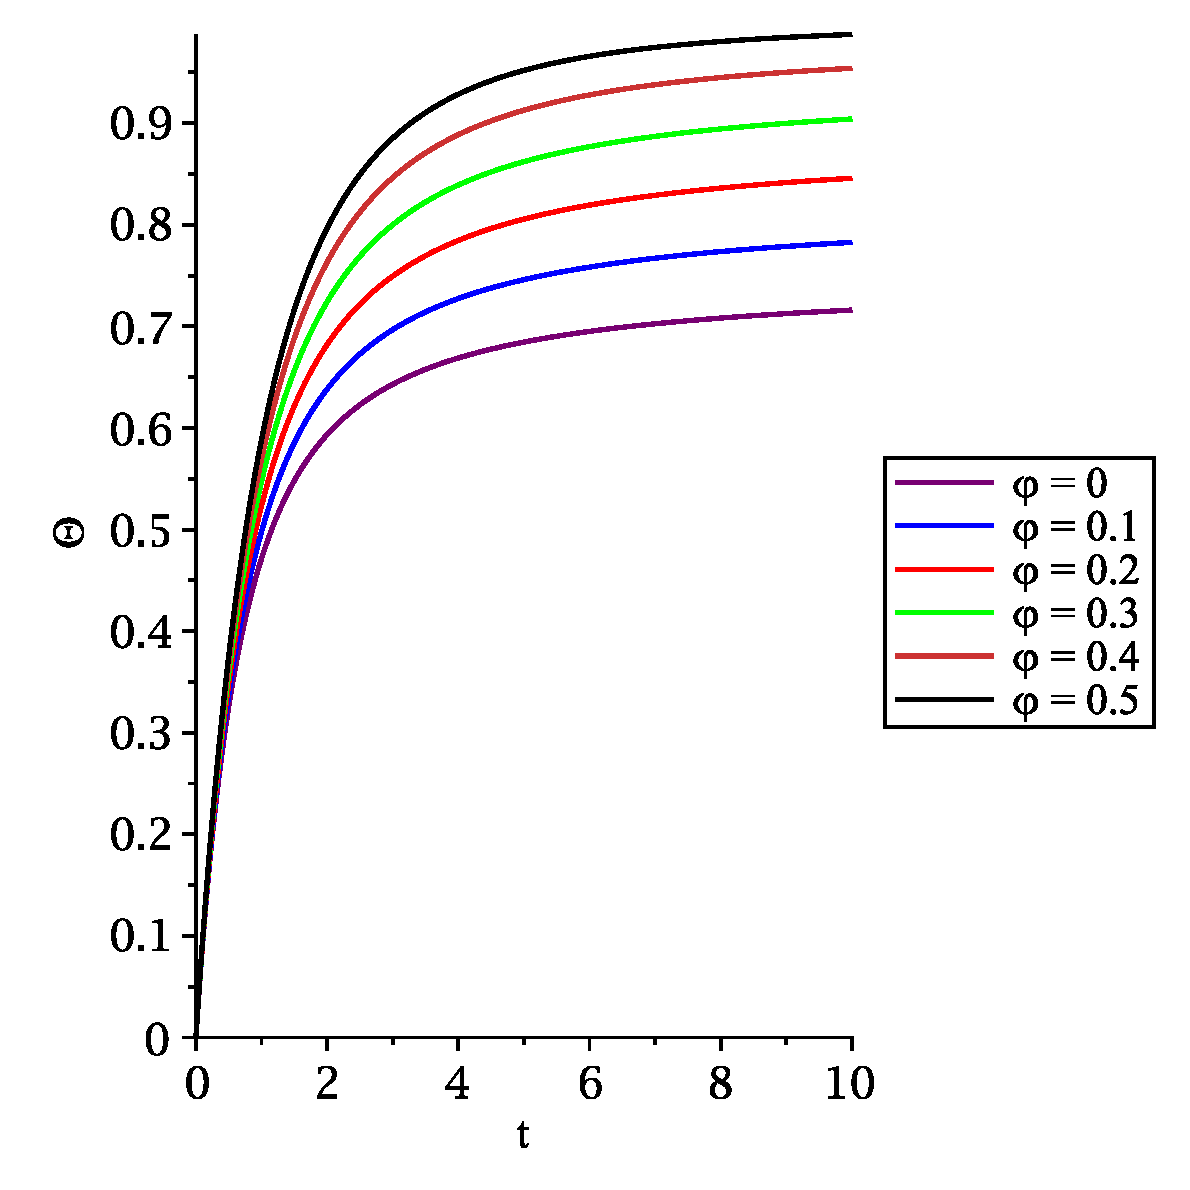
\includegraphics[scale = 0.35]{coverage_phi_01.eps}
	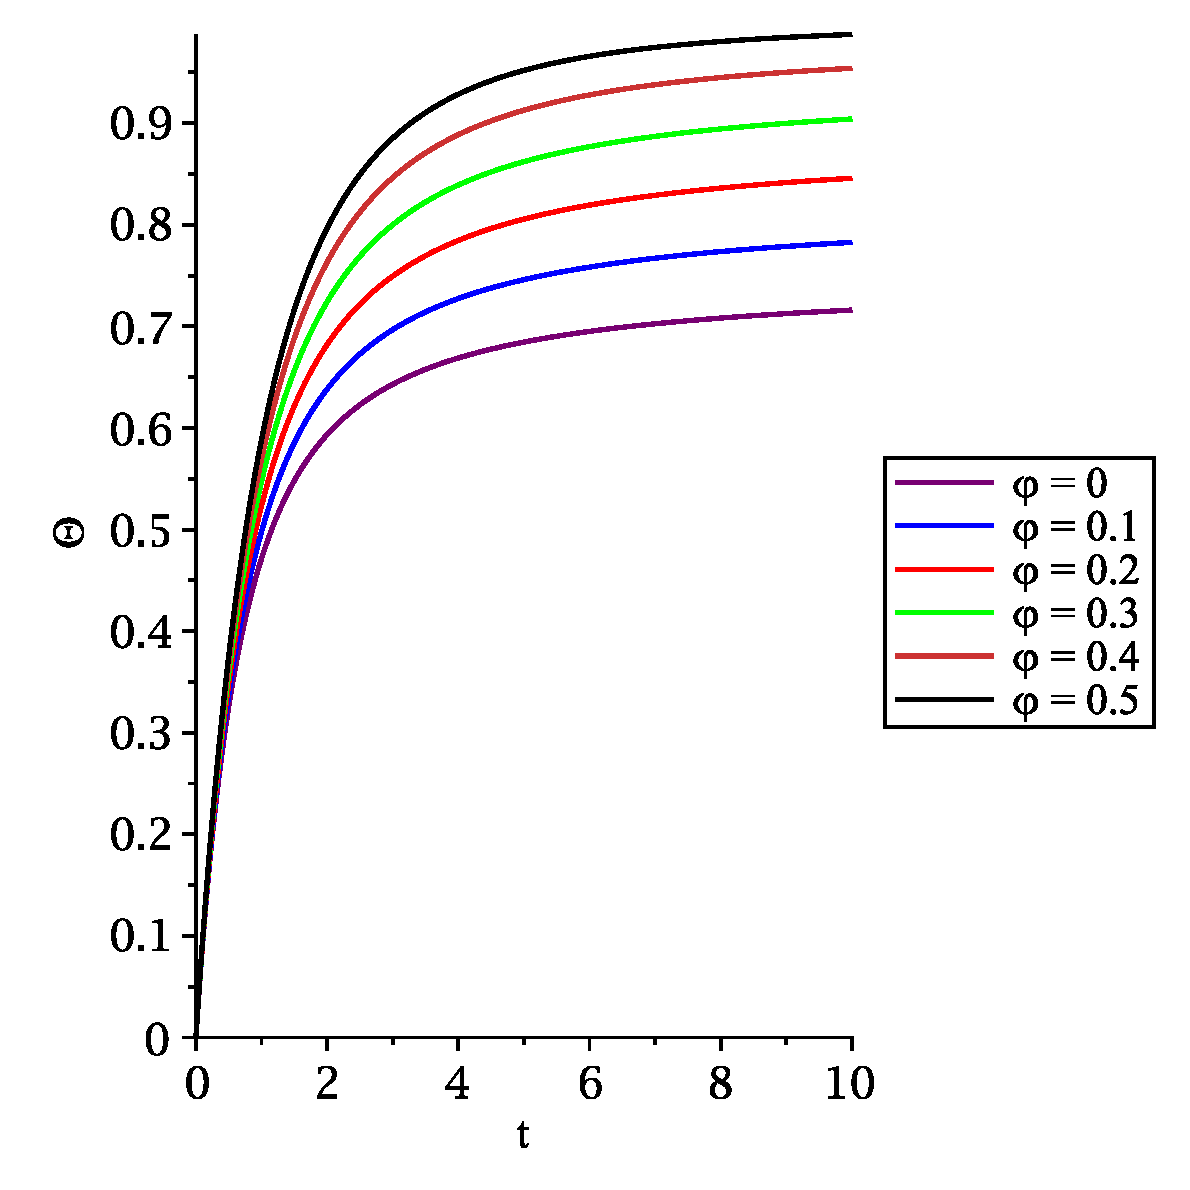
\includegraphics[width=\textwidth]{coverage_phi_01.eps}
	\caption{The coverage by cars}
	\label{fig:cp1}
\end{figure}\medskip

\newpage

In figure \ref{fig:cp2} we see the behaviour of the coverage for cars for 
values of $\phi$ between $0.5$ and $1$. As is to be expected, the coverage 
tends towards $1$ as $t$ increases. \bigskip

\begin{figure}[h!]
	\centering
	%	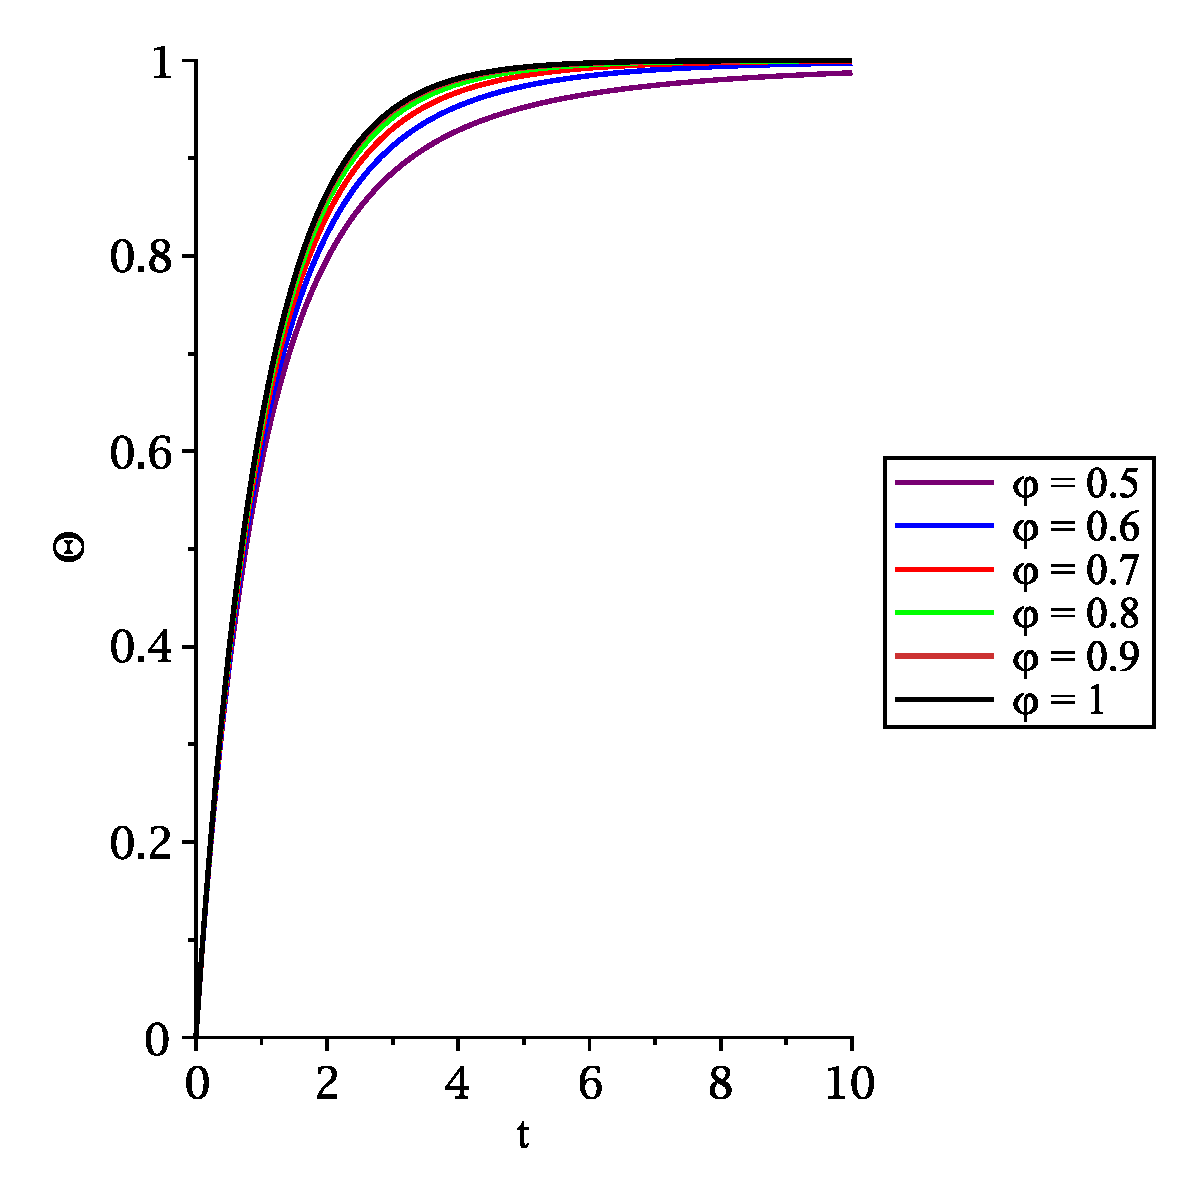
\includegraphics[scale = 0.35]{coverage_phi_02.eps}
	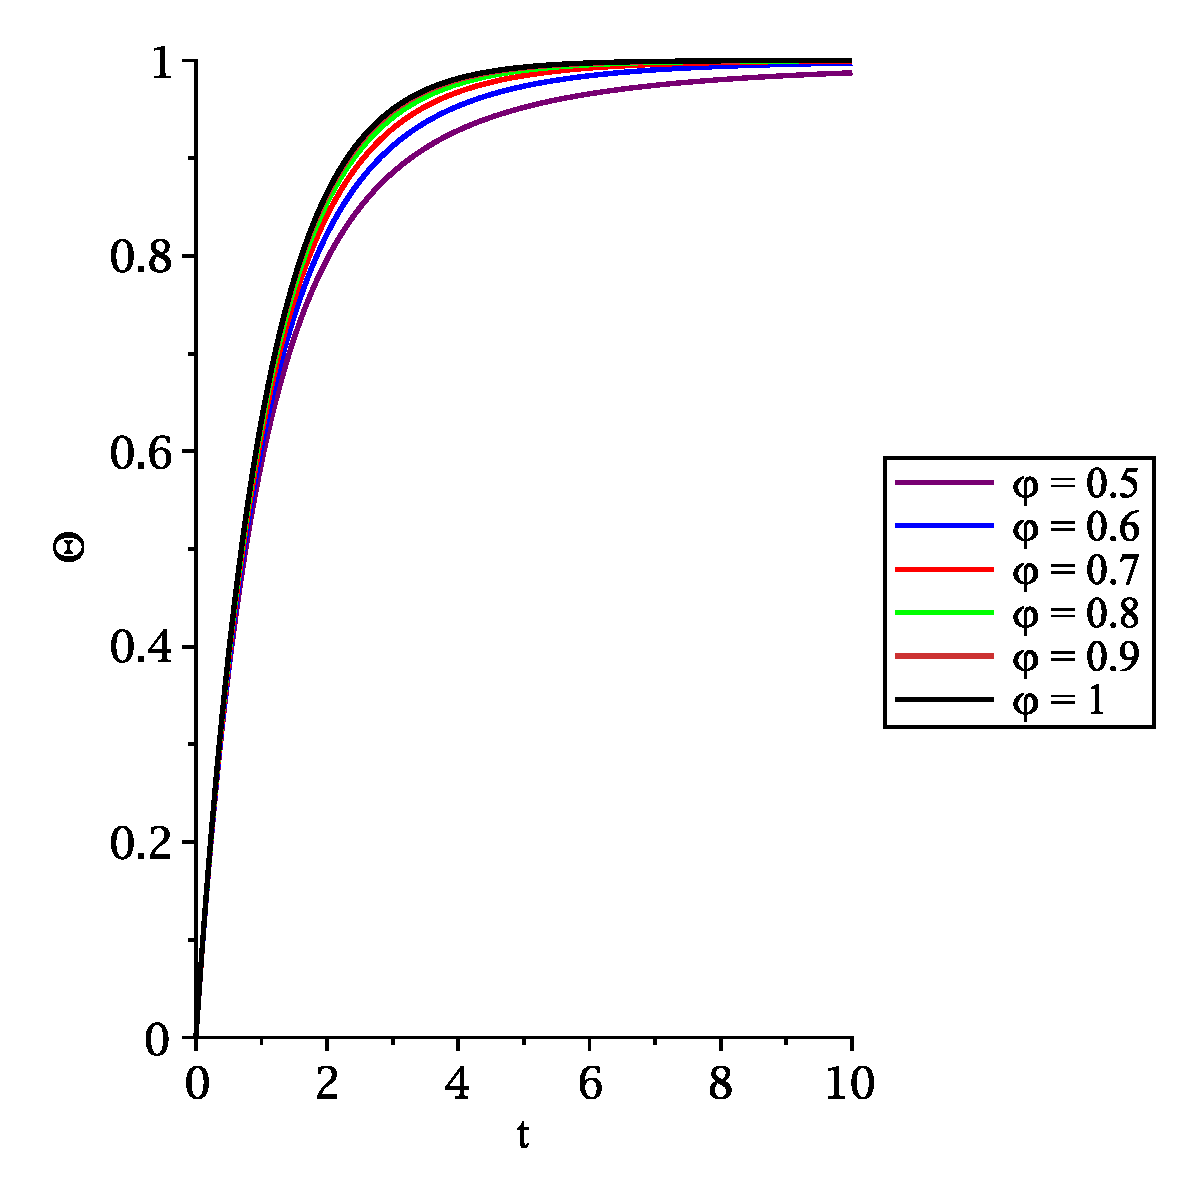
\includegraphics[width=\textwidth]{coverage_phi_02.eps}
	\caption{The coverage by cars}
	\label{fig:cp2}
\end{figure}\medskip

\newpage

We now consider the car coverage for $\phi = 1$. We first consider 
$F_{\phi}(t)$ when $\phi = 1$: \bigskip

\begin{eqnarray*}
	F_{\phi = 1}(t) & = & \exp \left( -2 \int_{0}^{t} \frac{(1 - e^{0})}{\tau} d\tau \right) \\\\
					& = & \exp \left( -2 \int_{0}^{t} \frac{(1 - 1)}{\tau} d\tau \right) \\\\
					& = & \exp \left( -2 \int_{0}^{t} \frac{0}{\tau} d\tau \right) \\\\
					& = & \exp \left( 0 \right) \\\\
					& = & 1
\end{eqnarray*}\medskip

making use of this we find: \bigskip

\begin{eqnarray*}
						\Theta_{\phi = 1}(t) & = & 1 - F_{\phi = 1}(t) e^{(1 - 2)t} \\\\
											 & = & 1 - e^{-t} \\\\
	\lim_{t \to \infty} \Theta_{\phi = 1}(t) & = & 1 - \lim_{t \to \infty} e^{-t} \\\\
											 & = & 1
\end{eqnarray*}\medskip

We now consider the car coverage for $\frac{1}{2} < \phi < 1$: \bigskip

\begin{eqnarray*}
	\lim_{t \to \infty} \Theta_{\phi}(t) & = & 1 - \lim_{t \to \infty} F_{\phi}(t) e^{(1 - 2 \phi)t} \\\\
										 & = & 1 - \lim_{t \to \infty} F_{\phi}(t) \cdot \lim_{t \to \infty} e^{-(2 \phi - 1)t} \\\\
										 & = & 1 - \lim_{t \to \infty} F_{\phi}(t) \cdot 0 \\\\
										 & = & 1 
\end{eqnarray*}\medskip

We now consider the car coverage for $\phi = \frac{1}{2}$. We first consider 
$F_{\phi}(t)$ when $\phi = \frac{1}{2}$: \bigskip

\begin{eqnarray*}
					 F_{\phi = 1/2}(t) & = & \exp \left( -2 \int_{0}^{t} \frac{(1 - e^{-\tau/2})}{\tau} d\tau \right) \\\\
									   & = & \exp \left( -2 \int_{0}^{t} \frac{1}{\tau} d\tau + 2 \int_{0}^{t} \frac{e^{-\tau/2}}{\tau} d\tau \right) \\\\
									   & = & \exp \left( -2 \int_{0}^{t} \frac{1}{\tau} d\tau\right) \cdot \exp \left( 2 \int_{0}^{t} \frac{e^{-\tau/2}}{\tau} d\tau \right) \\\\
									   & = & \exp \left( -2 \left. \ln(\tau) \right|_{\tau = 0}^{t} \right) \cdot \exp \left( 2 \int_{0}^{t} \frac{e^{-\tau/2}}{\tau} d\tau \right) \\\\
									   & = & \exp \left( - \left. \ln(\tau^2) \right|_{\tau = 0}^{t} \right) \cdot \exp \left( 2 \int_{0}^{t} \frac{e^{-\tau/2}}{\tau} d\tau \right) \\\\
									   & = & \exp \left( \ln\left( \frac{0}{t^2} \right) \right) \cdot \exp \left( 2 \int_{0}^{t} \frac{e^{-\tau/2}}{\tau} d\tau \right) \\\\
									   & = & \frac{0}{t^2} \cdot \exp \left( 2 \int_{0}^{t} \frac{e^{-\tau/2}}{\tau} d\tau \right) \\\\
	\therefore \quad F_{\phi = 1/2}(t) & = & 0
\end{eqnarray*}\medskip

and so we have: \bigskip

%\[
%	0 \leq F_{\phi = 1/2}(t) \leq 0 
%\]\medskip
%
%as $t \to \infty$, which implies: \bigskip
%
%\[
%	\lim_{t \to \infty} F_{\phi = 1/2}(t) = 0
%\]\medskip

\begin{eqnarray*}
	\Theta_{\phi = 1/2}(t) & = & 1 - F_{\phi = 1/2}(t) \\\\
%						   & = & 1 - F_{\phi = 1/2}(t) e^{0} \\\\
						   & = & 1 - 0 \\\\
						   & = & 1 
\end{eqnarray*}\medskip

hence if $\phi$ is at least $\frac{1}{2}$, then full coverage is achieved. In figure \ref{fig:cp3} 
we see the behaviour of the coverage for cars for values of $\phi$ between $0$ and $1$. \bigskip

\begin{figure}[h!]
	\centering
	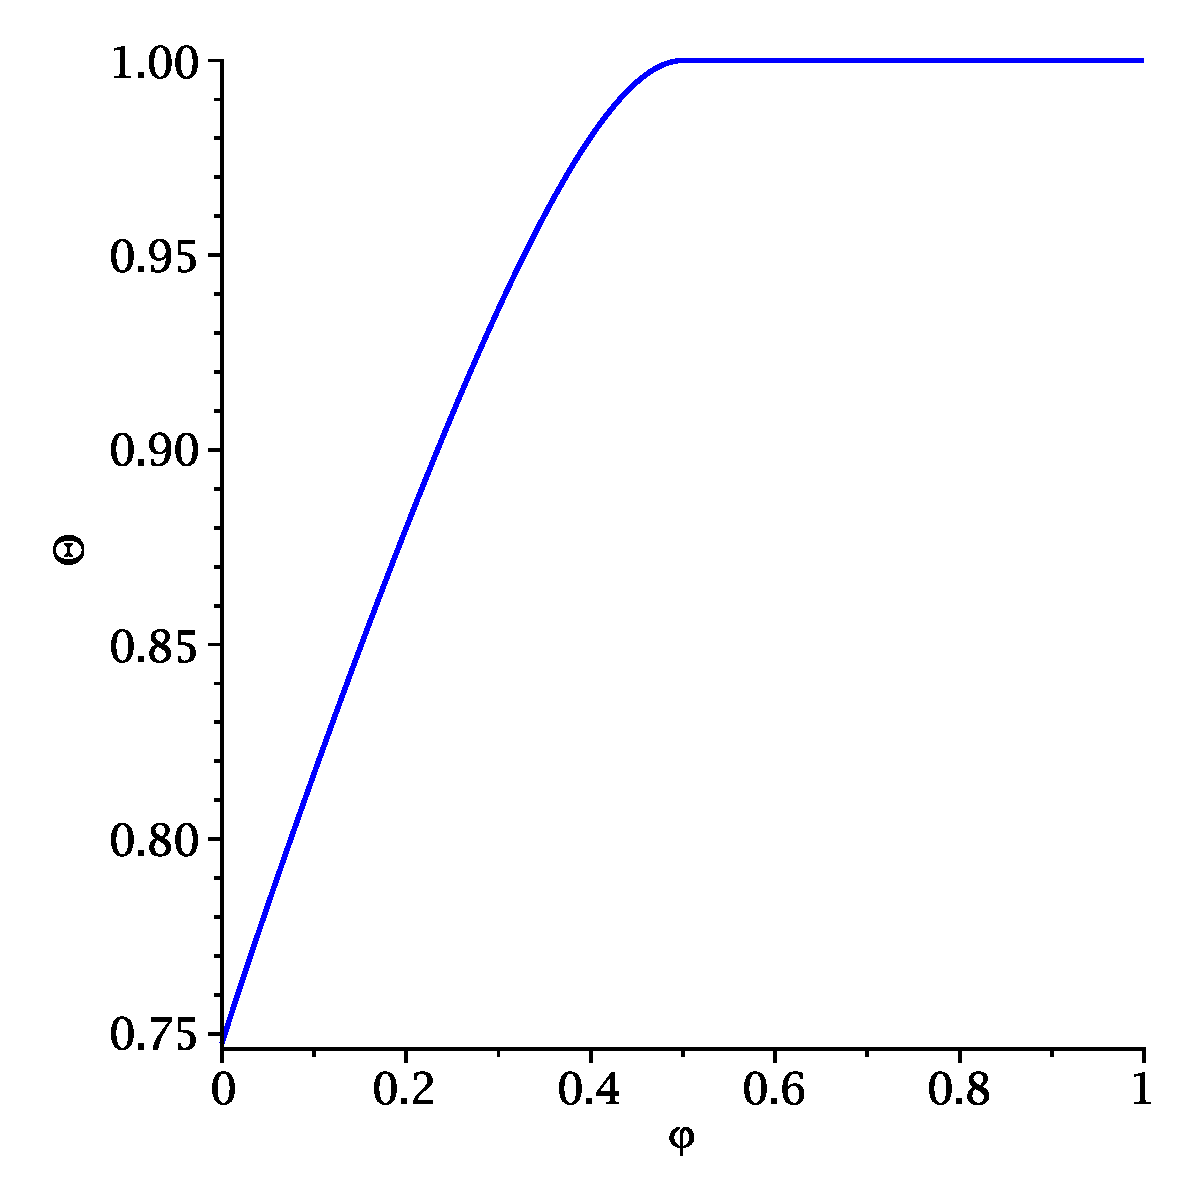
\includegraphics[scale = 0.35]{coverage_phi_03.eps}
%	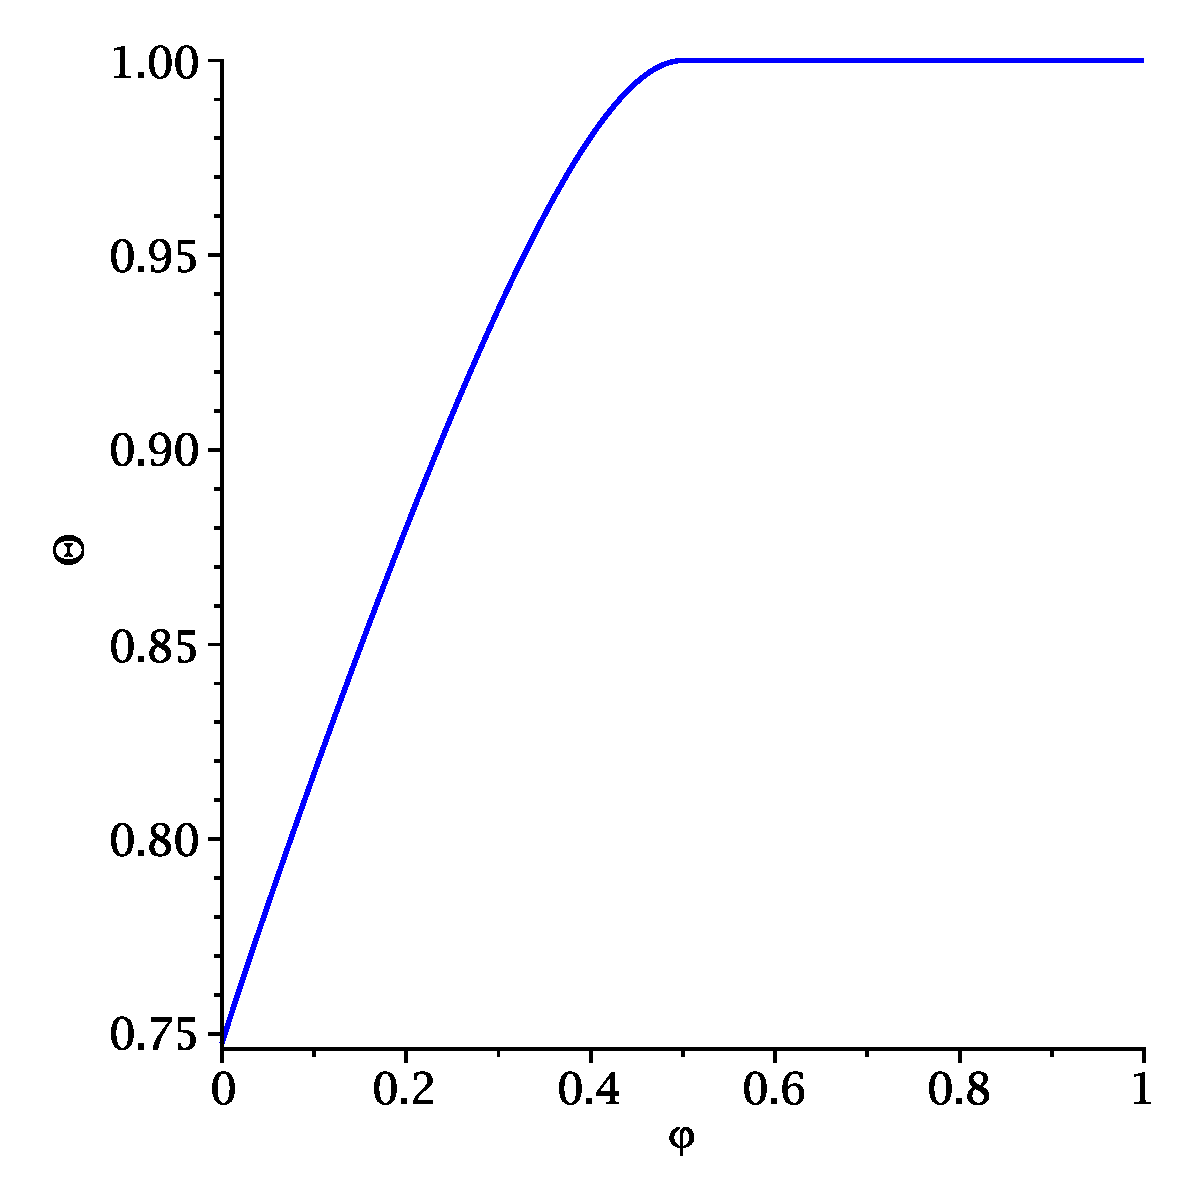
\includegraphics[width=\textwidth]{coverage_phi_03.eps}
	\caption{The coverage function as $t \to \infty$}
	\label{fig:cp3}
\end{figure}\medskip












\section{The reversible parking problem}

We now look at the reversible parking problem, where cars can both park and 
leave (see \cite{krapivsky1994collective}). In this version of the problem we 
assume that cars park at a rate of $k_{+}$ and leave at a rate of $k_{-}$. Thus 
far we have only considered the irreversible problem, which stops once the 
jamming limit has been reached. With the reversible problem we reach an 
equilibrium state when a balance is reached between the arrival rate $k_{+}$ 
and the leaving rate $k_{-}$. We define our rate equations for this case as 
follows, beginning with the $x < 1$ case: \bigskip

\[
	\frac{\partial P(x, t)}{\partial t} = -2 k_{-} P(x, t) + 2 k_{+} \int_{x + 1}^{\infty} P(y, t) dy  
\]\medskip

in which we have an adsorption ($+$) and a desorption ($-$) term. The adsorption 
term describes when a car parks within an interval of size $y > x + 1$, leaving a 
gap of length $x$, and this it can do in two different ways. The desorption term 
describes how a gap can be destroyed when any one of it's two neighbouring cars 
leaves. \bigskip

For the $x \geq 1$ case: \bigskip

\begin{eqnarray*}
	\frac{\partial P(x, t)}{\partial t} & = & -2 k_{-} P(x, t) + 2 k_{+} \int_{x + 1}^{\infty} P(y, t) dy \\\\
										&   &  -k_{+} (x - 1) P(x, t) + \frac{k_{-}}{\theta(t)} \int_{0}^{x - 1} P(y, t) P(x - 1 - y, t) dy 
\end{eqnarray*}\medskip

we have an additional two terms. The first describes how gaps of length greater 
than a car size are destroyed by arriving cars, with a rate $k_{+} (x - 1)$. The 
final term describes how two gaps separated by a car can form a larger gap when 
that car leaves. This term can be defined in terms of a gap-gap density function 
$P(y, z, t)$ which defines the density of neighbouring gaps of size $y$ and $z$ 
separated by a car. It can be defined as follows: \bigskip

\[
	P(y, z, t) = \frac{P(y, t) P(z, t)}{\theta(t)}
\]\medskip

In defining the gap-gap density function, we assume independence of the gap density 
functions, so that the distribution of two gaps separated by a single car is 
proportional to the product of the individual gap distributions. The coverage term 
in the denominator provides normalization. So the gap-gap density term above deals 
with the case where two neighbouring gaps, of size $y$ and $x - 1 - y$, separated 
by a single car, form a gap of size $x$ if the car separating the gaps leaves. \bigskip

From the above, it is clear that our condition for equilibrium is: \bigskip

\[
	\frac{\partial P(x, t)}{\partial t} = 0
\]\medskip

using the above rate equation we get: \bigskip

\begin{eqnarray*}
	-2 k_{-} P(x) + 2 k_{+} \int_{x + 1}^{\infty} P(y) dy & = & 0 \\\\
					2 k_{+} \int_{x + 1}^{\infty} P(y) dy & = & 2 k_{-} P(x) \\\\
							\int_{x + 1}^{\infty} P(y) dy & = & \frac{k_{-}}{k_{+}} P(x)
\end{eqnarray*}\medskip

using the substitution $P(x) = \beta e^{-\alpha x}$ we get: \bigskip

\begin{eqnarray*}
								  \int_{x + 1}^{\infty} \beta e^{-\alpha y} dy & = & \frac{k_{-}}{k_{+}} \beta e^{-\alpha x} \\\\
								  \beta \int_{x + 1}^{\infty} e^{-\alpha y} dy & = & \frac{k_{-}}{k_{+}} \beta e^{-\alpha x} \\\\
	\beta \left. \frac{ e^{-\alpha y} }{- \alpha} \right|_{y = x + 1}^{\infty} & = & \frac{k_{-}}{k_{+}} \beta e^{-\alpha x} \\\\
							  \frac{ e^{-\alpha} }{\alpha} \beta e^{-\alpha x} & = & \frac{k_{-}}{k_{+}} \beta e^{-\alpha x} \\\\
												  \frac{ e^{-\alpha} }{\alpha} & = & \frac{k_{-}}{k_{+}} \\\\
															 \alpha e^{\alpha} & = & \frac{k_{+}}{k_{-}} \\\\
\end{eqnarray*}\medskip

returning to our total coverage equation, and making the same substitution: \bigskip

\begin{eqnarray*}
														\int_{0}^{\infty} (x + 1) P(x) dx & = & 1 \\\\
								  \int_{0}^{\infty} x P(x) dx + \int_{0}^{\infty} P(x) dx & = & 1 \\\\
	\int_{0}^{\infty} x \beta e^{-\alpha x} dx + \int_{0}^{\infty} \beta e^{-\alpha x} dx & = & 1 \\\\
	\beta \int_{0}^{\infty} x e^{-\alpha x} dx + \beta \int_{0}^{\infty} e^{-\alpha x} dx & = & 1 \\\\
								\beta \left(\frac{1}{\alpha^2} + \frac{1}{\alpha} \right) & = & 1 \\\\
																	   \beta (1 + \alpha) & = & \alpha^2 \\\\
																					\beta & = & \frac{\alpha^2}{1 + \alpha} 
\end{eqnarray*}\medskip

which gives us for our equilibrium gap density function: \bigskip

\[
	P_{eq}(x) = \frac{\alpha^2}{1 + \alpha} e^{-\alpha x}
\]\medskip

We look next at the equilibrium coverage $\theta_{eq}$: \bigskip

\begin{eqnarray*}
	\theta_{eq} & = & \int_{0}^{\infty} P_{eq}(x) dx \\\\
				& = & \int_{0}^{\infty} \frac{\alpha^2}{1 + \alpha} e^{-\alpha x} dx \\\\
				& = & \frac{\alpha^2}{1 + \alpha} \int_{0}^{\infty} e^{-\alpha x} dx \\\\
				& = & \frac{\alpha^2}{1 + \alpha} \cdot \frac{1}{\alpha} \\\\
				& = & \frac{\alpha}{1 + \alpha} 
\end{eqnarray*}\medskip

And next we look at the function $\alpha \to \alpha e^{\alpha}$ on $(0, \infty)$: \bigskip

\begin{eqnarray*}
			 f(\alpha) & = & \alpha e^{\alpha} \\\\
	f^{\prime}(\alpha) & = & \alpha e^{\alpha} + e^{\alpha} \\\\
					   & = & (\alpha + 1) e^{\alpha} \\\\
					   & > & 0
\end{eqnarray*}\medskip

hence $f(\alpha)$ is strictly increasing on $(0, \infty)$. Therefore, if we were to 
graph the functions $y = f(\alpha)$ and $y = \frac{k_{+}}{k_{-}}$, they would meet 
in one and only one place, and hence there is a unique solution for 
$\alpha e^{\alpha} = \frac{k_{+}}{k_{-}}$. And also, as 
$\alpha e^{\alpha} = \frac{k_{+}}{k_{-}}$, if $\frac{k_{+}}{k_{-}} \to \infty$ 
then $\alpha e^{\alpha} \to \infty$ which implies $\alpha \to \infty$. In order to 
plot the equilibrium coverage as a function of $\frac{k_{+}}{k_{-}}$, we must first 
perform some manipulation: \bigskip

\begin{eqnarray*}
		 \alpha e^{\alpha} & = & \frac{k_{+}}{k_{-}} \\\\
	\ln(\alpha e^{\alpha}) & = & \ln \left( \frac{k_{+}}{k_{-}} \right) \\\\
	  \ln(\alpha) + \alpha & = & \ln \left( \frac{k_{+}}{k_{-}} \right) 
\end{eqnarray*}\medskip

Clearly, $\alpha$ dominates the left hand side as $\alpha \to \infty$, 
and hence: \bigskip

\[
	\alpha \approx \ln \left( \frac{k_{+}}{k_{-}} \right)
\]\medskip

putting this approximation for $\alpha$ into our expression for 
$\theta_{eq}$: \bigskip 

\begin{eqnarray*}
	\theta_{eq} & =       & \frac{\alpha}{1 + \alpha} \\\\
				& \approx & \frac{\alpha - 1}{\alpha} \quad \text{as } \alpha \to \infty \\\\
				& \approx & \frac{\ln(k_{+}/k_{-}) - 1}{\ln(k_{+}/k_{-})} \\\\
				& \approx & 1 - \frac{1}{\ln(k_{+}/k_{-})} 
\end{eqnarray*}\medskip

So we now have an approximation for the equilibrium coverage function as a 
function of $\frac{k_{+}}{k_{-}}$. In figure \ref{fig:ecf1} we see the behaviour 
of the equilibrium coverage function. We can see that $\theta_{eq}$ crosses $C_R$ 
(the red dashed line) as $\frac{k_{+}}{k_{-}}$ reaches approximately 50. \bigskip

\begin{figure}[h!]
	\centering
	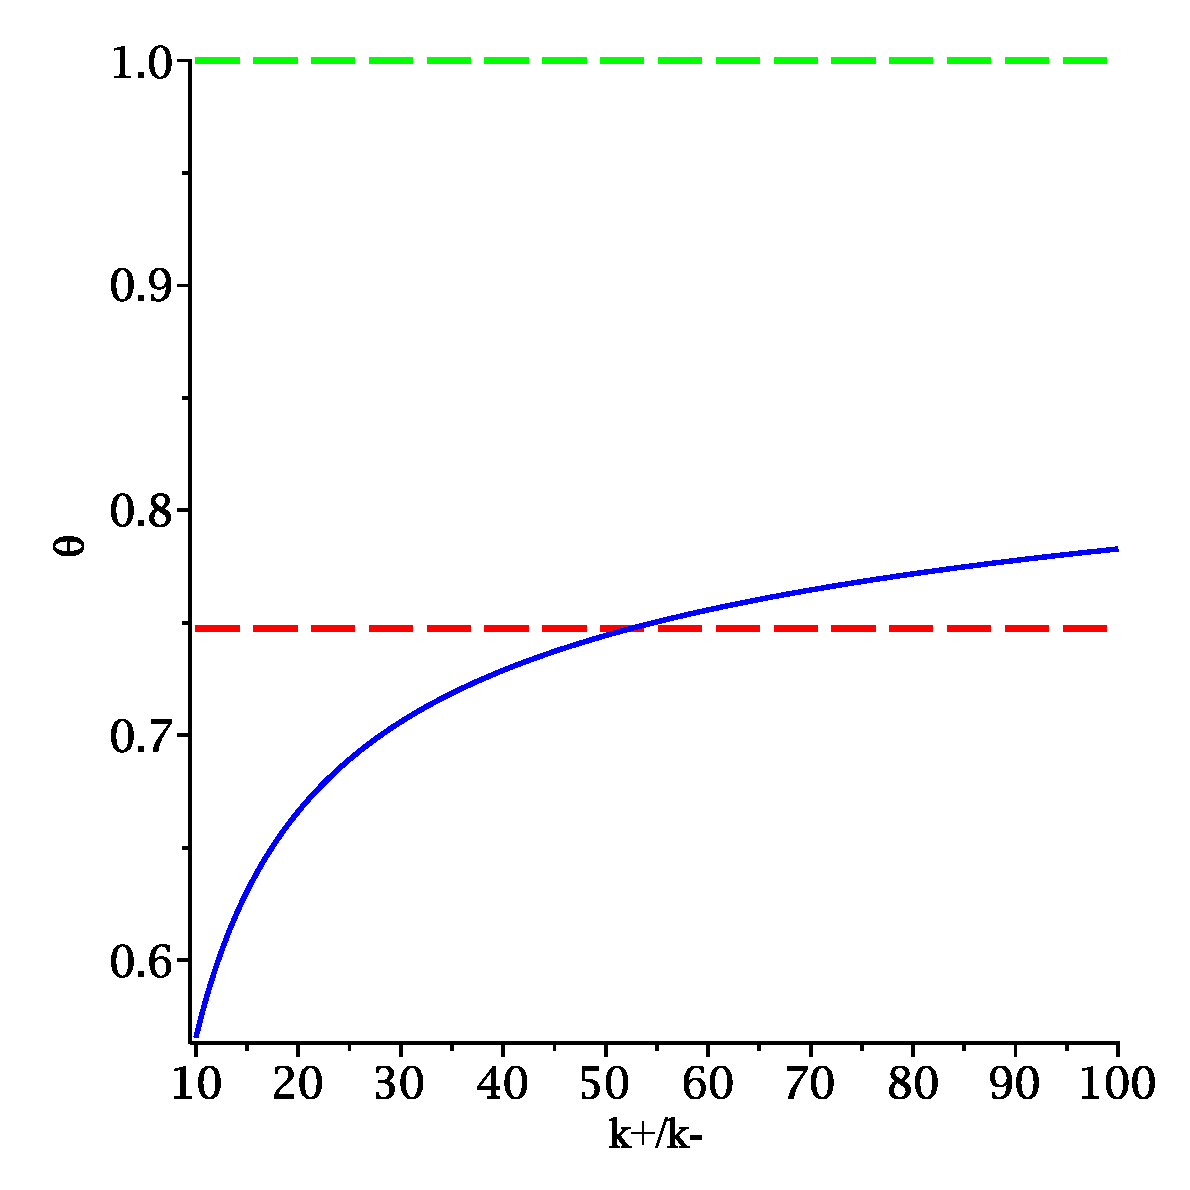
\includegraphics[scale = 0.35]{reversible_coverage_01.eps}
	%	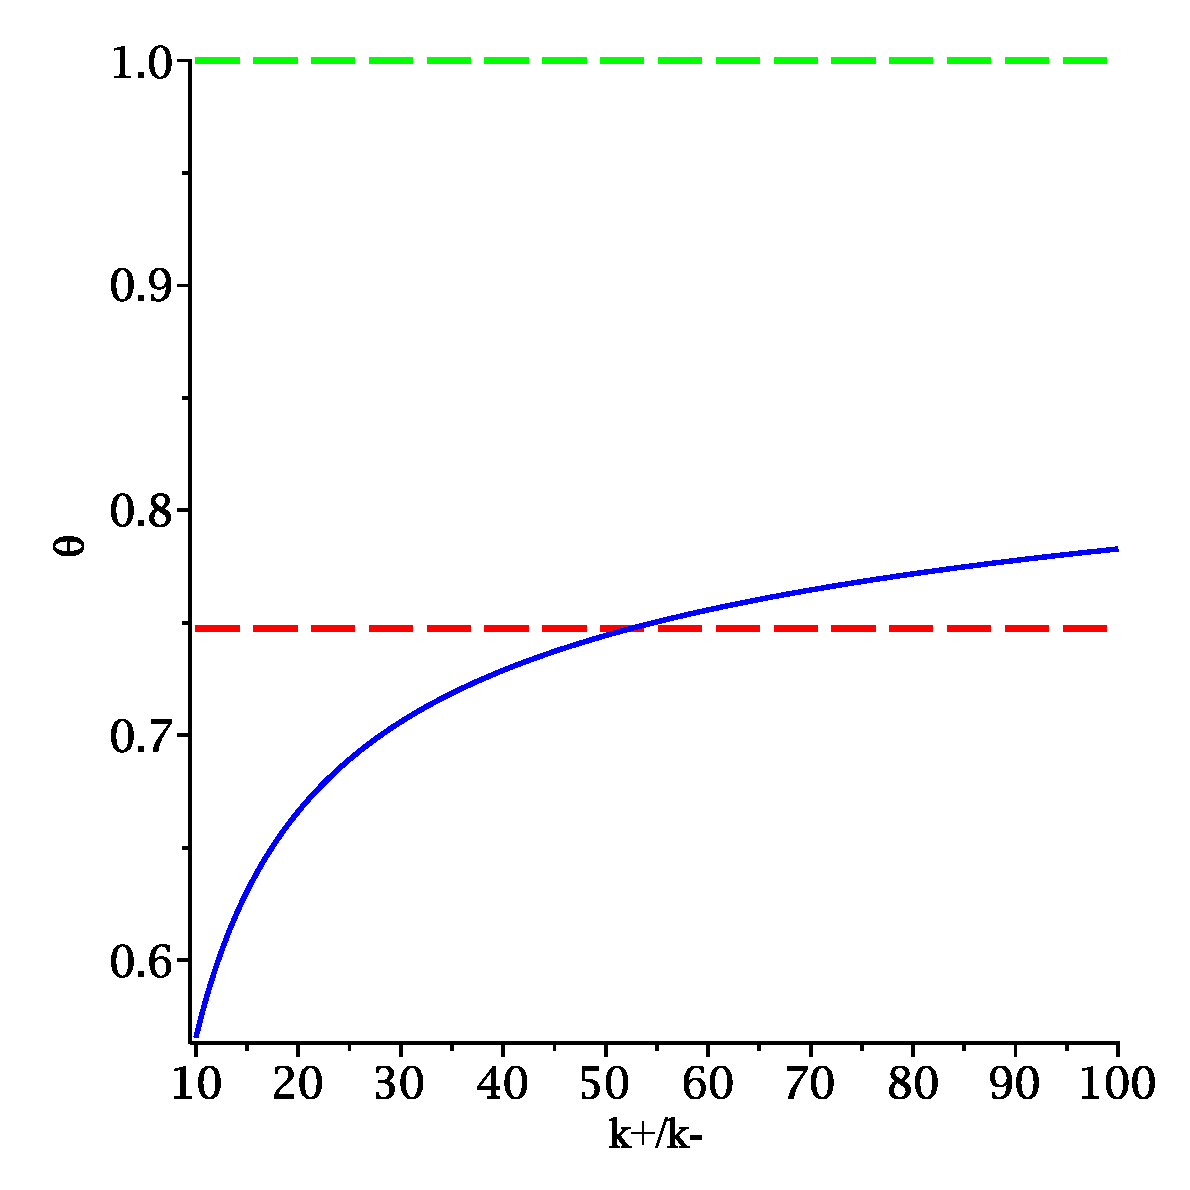
\includegraphics[width=\textwidth]{reversible_coverage_01.eps}
	\caption{The equilibrium coverage function}
	\label{fig:ecf1}
\end{figure}\medskip

In figure \ref{fig:ecf2} we see the behaviour of the equilibrium coverage 
function for a greater range of values of $\frac{k_{+}}{k_{-}}$. We can 
see that $\theta_{eq}$ continues to increase, albeit very slowly due to the 
logarithmic growth of the term involving $\frac{k_{+}}{k_{-}}$, towards $1$ 
(the green dashed line). \bigskip

\begin{figure}[h!]
	\centering
	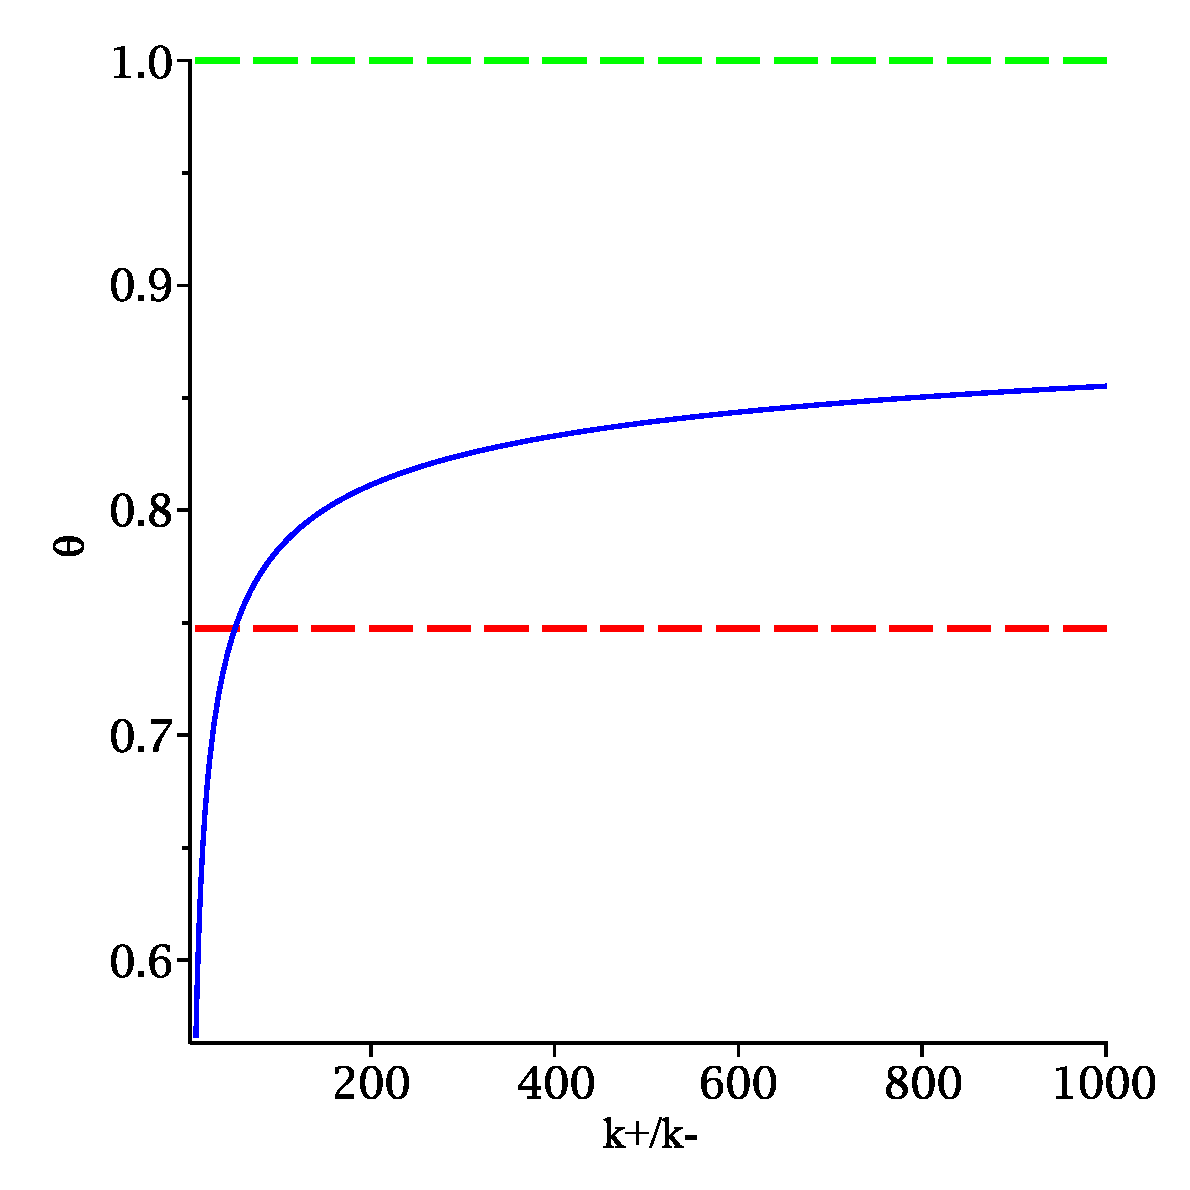
\includegraphics[scale = 0.35]{reversible_coverage_02.eps}
	%	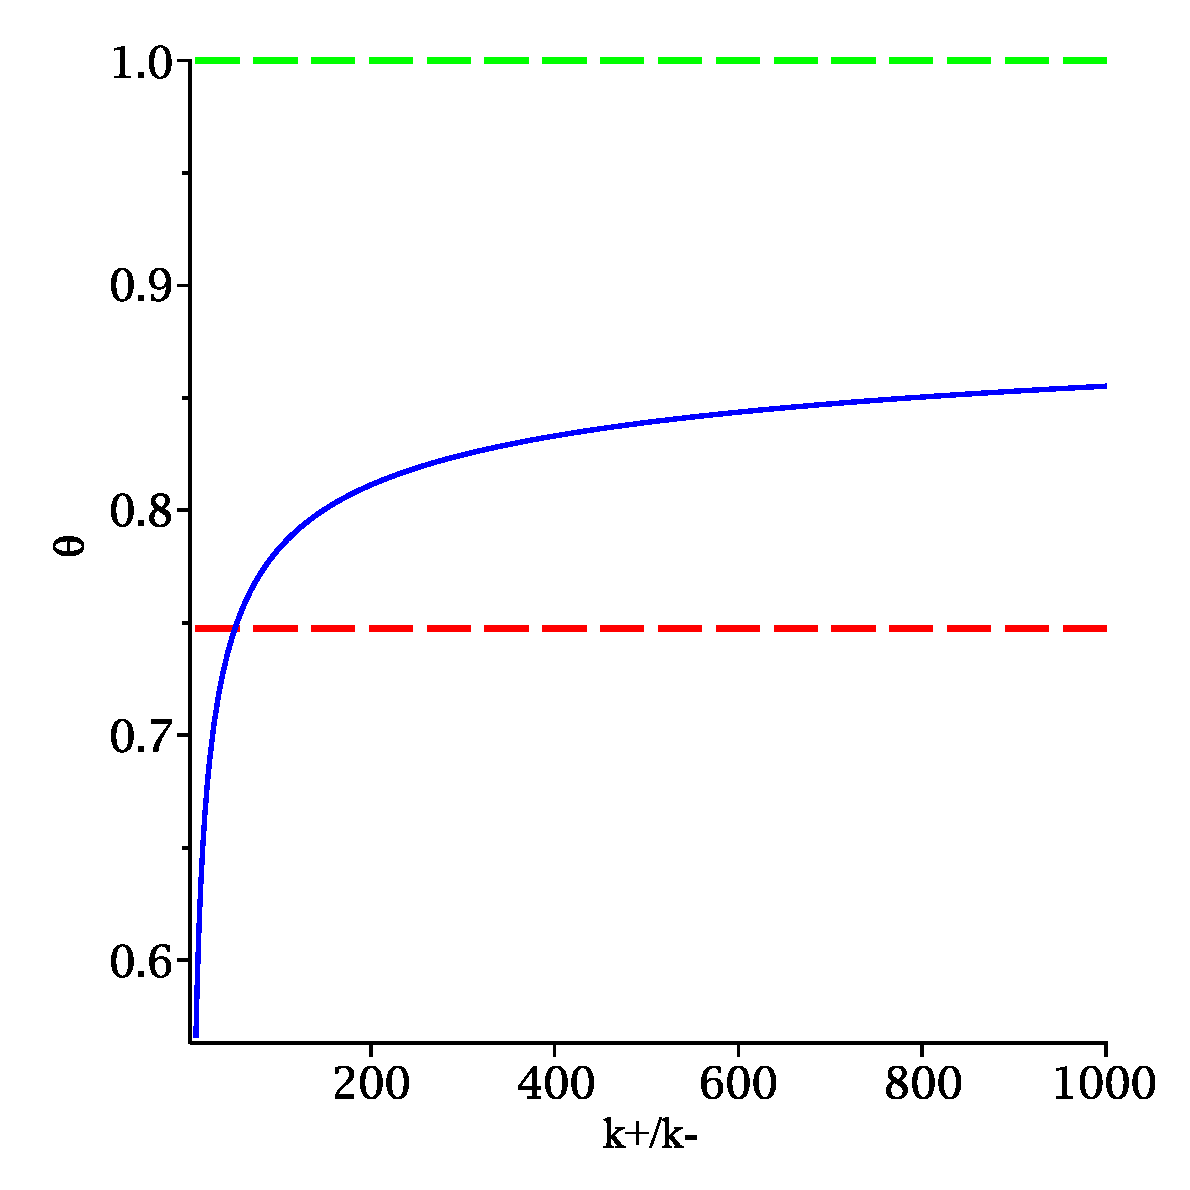
\includegraphics[width=\textwidth]{reversible_coverage_02.eps}
	\caption{The equilibrium coverage function}
	\label{fig:ecf2}
\end{figure}\medskip

It is easy to see from our approximation for the equilibrium coverage 
function that, as $\frac{k_{+}}{k_{-}} \to \infty$, 
$\ln\left(\frac{k_{+}}{k_{-}}\right) \to \infty$, and hence: \bigskip

\[
	\theta_{eq} \to 1 \quad \text{as } \frac{k_{+}}{k_{-}} \to \infty
\]\medskip

Where $k_{-} \to 0$, we have $\frac{k_{+}}{k_{-}} \to \infty$, and 
$\theta_{eq} \to 1$. So as $k_{-}$ gets closer to $0$, for example 
in the case where we can control desorption, the process tends towards 
full coverage. But in the case where $k_{-} = 0$, our problem collapses 
into the standard parking problem, and coverage falls back to $C_R$.











\section{Remarks}

As with the kinetic approach, we have successfully modelled the process with 
respect to it's time evolution, and with some generalizations. \bigskip

These solutions are even more satisfying than the kinetic approach because 
the assumptions of each extend the assumptions of the kinetic approach: \bigskip

\begin{itemize}
	\item \textbf{Kinetic Approach:} time evolution of parking cars
	\item \textbf{Overlap Approach:} time evolution of parking exclusion zones
	\item \textbf{Reversible Approach:} time evolution of cars that park and 
	leave at different rates
\end{itemize}\medskip

This can be seen in the construction of each of their rate equations, 
where the rate equations for each generalization builds on the rate 
equations of the kinetic approach by adding extra terms reflecting 
the extra sophistication. \bigskip










